% ------------------------------------------------------------------------
% file `uaa_radicaux_pythagore_trigonometrie-exercise-10-exercise-body.tex'
%   in folder `xsim/'
%
%     exercise of type `exercise' with id `10'
%
% generated by the `exercise' environment of the
%   `xsim' package v0.20c (2021/02/03)
% from source `uaa_radicaux_pythagore_trigonometrie' on 2021/12/01 on line 180
% ------------------------------------------------------------------------
    Le sol du garage de la maison de Boris se trouve à 2,30m sous le rez-de-chaussée.
    La maison est en recul de 7m par rapport au trottoir. Le croquis ci-dessous illustre
    cette situation. Calcule l'amplitude de l'angle de la rampe d'accès au garage et exprime la pente
    de cette rampe en pourcentage. Ecris ton raisonnement.\\
    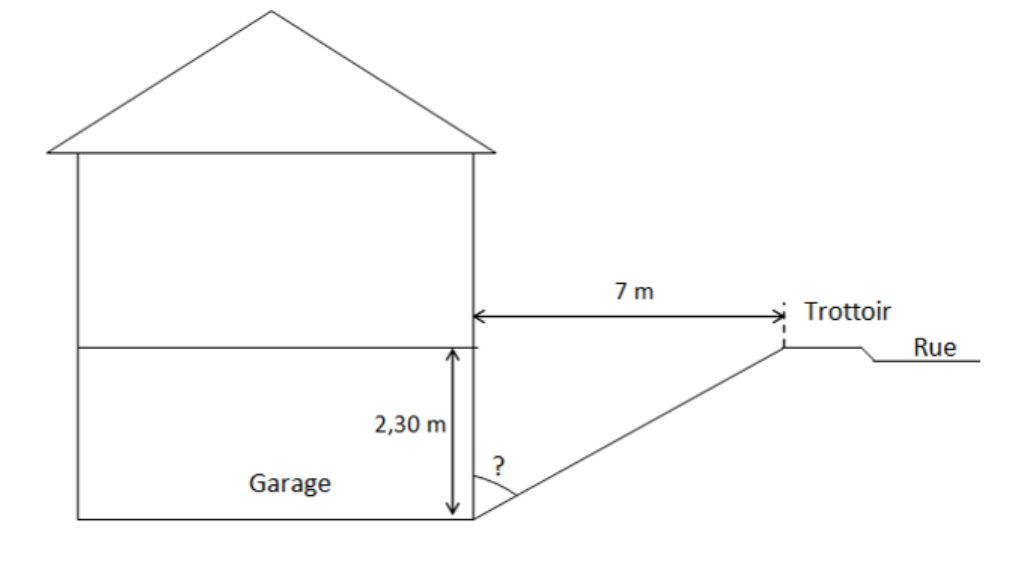
\includegraphics[width=15cm]{img/Q15.png}

